\documentclass[aspectratio=169]{beamer}

\usepackage[spanish,es-nodecimaldot]{babel}
\usepackage[utf8]{inputenc}
\usepackage[T1]{fontenc}
\usepackage{graphicx}
\usepackage{booktabs}
\usepackage{xcolor}
\usepackage{hyperref}
\usepackage{tikz}

\usetheme{Madrid}
\setbeamertemplate{navigation symbols}{}
\setbeamertemplate{footline}{}
\graphicspath{{../Exploracion_Datos/Figuras/}{../Informe_Tecnico/}}

\title{Exploración de datos 1D y 2D}
\subtitle{Guía N°1}
\author{Gianfranco Giannoni}
\institute{Herramientas para Ciencias de Datos\\
Docente: Michael Miranda\\
Universidad Tecnológica Metropolitana}
\date{22 de octubre de 2026}

\begin{document}

\begin{frame}
\titlepage
\begin{tikzpicture}[remember picture,overlay]
\node[
  anchor=north west,
  xshift=1.1cm,
  yshift=-0.1cm
] at (current page.north west) {
\includegraphics[width=1.9cm]{logo_utem.png}};
\end{tikzpicture}
\end{frame}

\begin{frame}{Objetivo y fuentes}
\begin{itemize}
\item Explorar una señal 1D y una imagen 2D.
\item Documentar procedencia, unidades, representación y calidad.
\item Identificar limitaciones antes de usar inteligencia artificial.
\end{itemize}
\vspace{.4cm}
\begin{block}{Fuentes}
\begin{itemize}
\item Audio musical GTZAN, WAV mono, 22050 Hz, 30 s, licencia CC0.
\item Termografía fotovoltaica, JPEG RGB de 640$\times$512, licencia CC0.
\end{itemize}
\end{block}
\end{frame}

\begin{frame}{Señal 1D: representación}
\begin{itemize}
\item Las muestras se representan como \(x[n]\).
\item El eje temporal se calcula con \(t[n]=n/f_s\).
\item \(f_s=22050\) Hz y el paso es \(4.5351\times10^{-5}\) s.
\item La amplitud graficada está normalizada digitalmente.
\item No representa presión acústica calibrada.
\end{itemize}
\end{frame}

\begin{frame}{Señal 1D: resultados}
\centering
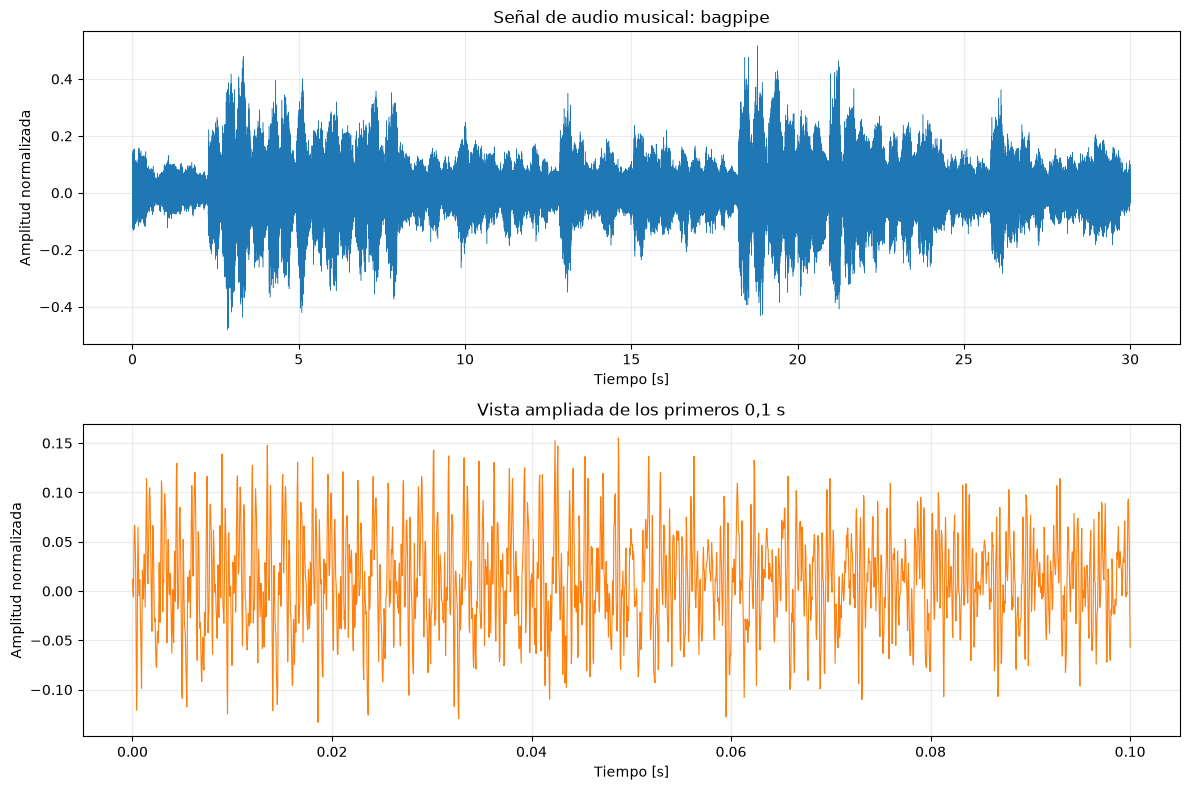
\includegraphics[width=.96\textwidth,height=.76\textheight,keepaspectratio]{Figura 1A.png}
\end{frame}

\begin{frame}{Imagen 2D: representación}
\begin{itemize}
\item Arreglo \(I[y,x,c]\) de forma \((512,640,3)\).
\item Coordenadas espaciales en píxeles.
\item Tres canales: rojo, verde y azul.
\item Tipo \texttt{uint8}, rango codificado esperado 0--255.
\end{itemize}
\end{frame}

\begin{frame}{Imagen 2D: resultados}
\centering
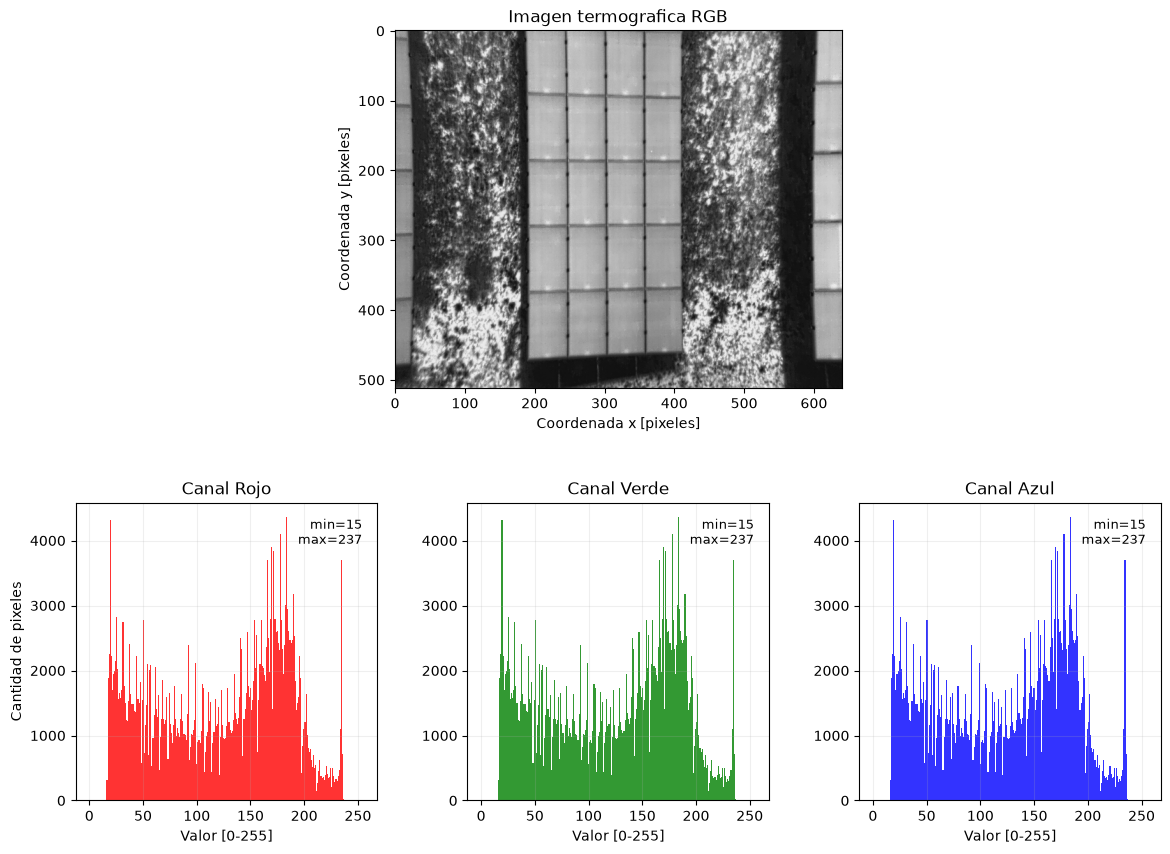
\includegraphics[width=.96\textwidth,height=.76\textheight,keepaspectratio]{Figura 1B.png}
\end{frame}

\begin{frame}{Controles de calidad}
\begin{table}
\centering
\small
\begin{tabular}{lll}
\toprule
 & \textbf{Audio} & \textbf{Imagen}\\
\midrule
Dimensión & 661500 muestras & 640$\times$512$\times$3\\
Formato & WAV PCM int16 & JPEG RGB uint8\\
Rango & -15756 a 16956 & 15 a 237\\
Valores inválidos & 0 no finitos & 0 fuera de rango\\
Consistencia & paso temporal constante & ningún canal constante\\
\bottomrule
\end{tabular}
\end{table}
\end{frame}

\begin{frame}{Metadatos y limitaciones}
\begin{columns}
\column{.48\textwidth}
\textbf{Audio}
\begin{itemize}
\item Faltan micrófono, distancia y nivel de grabación.
\item Una pista no representa toda la música.
\end{itemize}
\column{.48\textwidth}
\textbf{Imagen}
\begin{itemize}
\item Faltan calibración radiométrica y emisividad.
\item JPEG puede introducir artefactos.
\item Faltan condiciones térmicas y eléctricas.
\end{itemize}
\end{columns}
\end{frame}

\begin{frame}{Pregunta de inteligencia artificial}
\begin{block}{Pregunta}
¿Puede un modelo identificar una posible anomalía térmica en un panel
fotovoltaico manteniendo pocos falsos negativos frente a una inspección experta?
\end{block}
\textbf{Se necesitan:}
\begin{itemize}
\item etiquetas de anomalía, ubicación y severidad;
\item temperatura radiométrica y mediciones eléctricas de referencia;
\item condiciones de captura completas;
\item validación experta y métricas de sensibilidad, especificidad y falsos
negativos.
\end{itemize}
\end{frame}

\begin{frame}{Conclusiones}
\begin{itemize}
\item La señal 1D describe variación temporal; la imagen 2D describe
distribución espacial y canales.
\item Ambas fuentes se cargaron y visualizaron reproduciblemente.
\item La calidad del archivo no implica calibración física.
\item Antes de entrenar un modelo se deben completar metadatos, etiquetas y
referencias de medición.
\end{itemize}
\end{frame}

\end{document}
